\chapter{Implementation}

This chapter aim to elaborate on the implementation details of the project undertaken in order to establish a platform which will allow for evaluating different classification algorithms and subsequently drawing conclusions from such evaluation.

\section{Overview}

The system consists of the number of independent components, further described in subsequent sections. Each of this components is expected to provide a certain set of methods, later referred to as APIs. As long as these requirements are met, those modules can easily be replaced or modified provided they adhere to the same interface.

This modularity enabled me to work concurrently on different parts of the system without any significant interference. It also contributed to the scalability and parallelisation of the system, where crawlers and classifiers could easily be distributed across different servers and still perform adequately.

The system is split into three primary components: core infrastructure for handling Twitter messages, database connections and scores; a crawler which was used to create the data set and a set of classifiers with a generic runner. The architecture of these components is explained in more detail in the following sections.

\section{Infrastructure}

In order to avoid code repetition and discrepancies between different classification methods, I implement a set of common interfaces which are then used by higher-level implementations in order to facilitate access to the data set, feature reduction algorithms, running the classification algorithms and computing performance scores.

The system is kept modular by isolating commonly used abstractions in the \verb|common| folder. It contains implementations of \verb|Score| and \verb|Tweet| classes, which provide interfaces for working with individual Twitter messages and cumulative classification scores.

The \verb|Tweet| class assumes access to the data set through a set of APIs provided by \verb|ActiveRecord|. This allows for immediate support for multiple relational data stores. Through the use of \verb|ActiveModel| this support can be extended to any other data source, such as \verb|Hadoop|\footnote{\url{http://hadoop.apache.org/}} or even plain text files, as long as they adhere to a predefined interface.

\subsection{External Dependencies}

I yuse \verb|Bundler|\footnote{\url{http://gembundler.com/}} to manage application's dependencies across multiple machines. Having specified these dependencies, \verb|Bundler| will keep track of required gems and their version numbers in order to establish a consistent execution environment, regardless of the machine at which the application is run.

\subsection{Storage}

An SQLite database was used to store both training and test data. Working with a relational database rather than files allowed for easier formatting and querying the data, especially with respect to filtering out messages of certain language or sentiment.

Messages are stored in a single \verb|tweets| table with the following columns: \verb|status_id|, \verb|language|, \verb|text| and \verb|json|, where:

\begin{itemize}
  \item \verb|status_id| is a unique Twitter status identifier
  \item \verb|language| is an ISO 639-1 coded language of the message
  \item \verb|text| is the full text of the status message
  \item \verb|json| is the original JSON response as received from the Twitter API.
\end{itemize}

The original JSON response is retained so that parameters other than \verb|status_id|, \verb|language| or \verb|text| could be recovered if necessary. I de-normalise the schema and introduce indexes to be able to efficiently filter out records by any of aforementioned parameters. Consistency is maintained because records are not modified after they have been added to the database.

\section{Twitter Crawler}

Before any analysis could be carried out it was necessary to gather enough training and test data.

For this purpose, I built a simple crawler which queried Twitter Search API\footnote{\url{http://dev.twitter.com/doc/get/search}} and persisted the results in a local database for further processing and analysis.

In order to avoid having to interact with Twitter API\footnote{\url{http://dev.twitter.com/doc}} directly, I used an open source Twitter gem\footnote{Gems are self-contained packages for distributing Ruby programs and libraries.} which implements OAuth authentication as well as easy API access in Ruby\footnote{\url{https://github.com/jnunemaker/twitter/}}.

There are two features of the Twitter API that are crucial to the operation of our crawler:

\begin{itemize}
  \item {\bf Language filter.} Passing an optional \verb|lang| parameter restricts tweets to a given language, given by an ISO 639-1 code.
  \item {\bf Attitude filter.} Querying for \verb|:)| and \verb|:(| returns tweets with positive and negative attitude respectively. This feature is not documented in the Search API, but has been announced\footnote{\url{http://twitter.com/twitter/status/2262419764}} by Twitter and is listed amongst other search operators\footnote{\url{http://search.twitter.com/operators}}.
\end{itemize}

The crawler will therefore carry out a separate query for each sentiment class in each language. For example, when retrieving positive tweets in English, the wrapper would send a \verb|HTTP GET| request to \verb|http://search.twitter.com/search.json?q=:)&lang=en|.

The result of such request is then parsed and each message is instantiated as a \verb|Tweet| object, later persisted by invoking the \verb|save| method provided by \verb|ActiveRecord|. A utility method \verb|Tweet#parse| was written to make this process simpler.

The crawler was then run in the cloud using Amazon Elastic Cloud Computing\footnote{\url{http://aws.amazon.com/ec2/}} service (EC2), part of the Amazon Web Services infrastructure. Running the crawler on a remote server instead of on my local machine mitigated the risks associated with both connection and hardware failures. The database was regularly downloaded and backed up to my personal Dropbox account to avoid potential data loss.

\subsection{Limitations}

Since results filtered with the \verb|lang| parameter are limited to last 7 days and the API itself imposes a rate limit, I needed to run the crawler over a few weeks with idle intervals of 10 minutes between each run (which involves 10 different queries, two for each of the five languages) to avoid exceeding said limit. Since Twitter reserves the right to block applications which do not comply to its terms of service, it was critically important that these limits are respected in order to successfully complete the project.

\section{Feature Reduction}

There are several properties, some unique to Twitter, that can be taken advantage of in order to reduce the feature space.

\begin{itemize}
  \item \textbf{Case sensitivity.} In order to avoid differentiating between spelling variations of the same word (e.g. \verb|Love|, \verb|love| or even \verb|lOvE|), all documents are converted to lower case first.

  \item \textbf{Usernames.} Since Twitter users often direct messages to each other by prepending other people's Twitter handles with an \verb|@| symbol, I introduce the \verb|USERNAME| equivalence class token, replacing all words that start with the \verb|@| symbol.

  \item \textbf{Links.} Similarly, Twitter users often include links in their messages. I therefore introduce another equivalence class which maps all URLs to the \verb|URL| token.

  \item \textbf{Repeated letters.} Due to the prominent use of casual language on Twitter, repeated letters are often used as a form of emphasis (e.g. writing \verb|loooooooove| to mean \verb|love|). I therefore ignore all duplicate letters after the first two occurrences (i.e. mapping \verb|loooooooove| to \verb|loove|).
\end{itemize}

This process, also known as feature extraction, is important since classification can be done more accurately in a reduced rather than original space.

All these reductions are performed on-the-fly using regular expressions, the list of which is defined in the \verb|Tweet#reductions| method so that it could be easily extended if necessary.

\section{Testing and Evaluation}

In order to maintain the consistency of testing between different classification methods, the \verb|Classifier::Base| class provides a unified way of performing and evaluating classifications using k-fold cross validation. By default a 10-fold cross-validation is used, but the library allows to change the number of folds if necessary.

Firstly, the crawler queries the database to collect two data sets for each language--one containing only positive and one only negative tweets. It also initiates a \verb|Score| instance. New data points can then added using the \verb|Score#add| method, which compares sentiment passed on from the classifier with tweet's original label and increments appropriate counters. These counters can then be used to calculate precision and recall for individual folds as well as an average cumulative result.

I use the following definitions when computing aforementioned metrics:

\begin{itemize}
  \item $\textrm{precision}(c) = \frac{\textrm{\# of documents correctly classified as `c'}}{\textrm{total \# of documents classified as `c'}}$
  \item $\textrm{recall}(c) = \frac{\textrm{\# of documents correctly classified as `c'}}{\textrm{total \# of documents}}$
\end{itemize}

Where $c$ in the equations above stands for the sentiment class, i.e. \verb|positive| or \verb|negative|.

\verb|Score| class also implements two helper functions: \verb|summary| and \verb|latex|. The former outputs the results held in the \verb|Score| instance in a human-readable form: stating which classifier was used, which language is being evaluated as well as individual and cumulative performance metrics. The latter outputs the same results in the {\LaTeX} format, which can be directly embedded in documents such as this dissertation.

Instances of the \verb|Score| class can also be easily added together with the \verb|Score#+| method, which overrides the default addition operator. The new score inherits the label, classifier and language of the left-most operand and merges all internal counters.

Individual implementations, such as \verb|Classifier::NaiveBayes|, need only to extend the \verb|Classifier::Base| class to inherit most of its functionality, whilst implementing their own classification techniques. This can be achieved by calling the \verb|evaluate| method and passing a block of code containing the classification procedure. Test and training data along with the \verb|Score| object are passed as arguments to this block and do not have to be instantiated in each implementation. Each of these classes can change the default parameters set by \verb|Classifier::Base|, including the list of languages to be evaluated, the number of tweets per language or the number of folds performed.

\section{Classifiers}

This section outlines the implementation of various sentiment classification techniques, including the machine learning techniques to be evaluated. Since most classifiers have been implemented using readily-available libraries, it is primarily concerned with changes that needed to be made in order to use these libraries in the project, includes normalising input/output differences between algorithms and additional parameters that might affect evaluation consistency.

\subsection{Baseline}

As a baseline, I decided to use a keyword-based dictionary count with a list of 405 positive and 500 negative keywords\footnote{\url{http://www.liwc.net/}}, an approach that has been successfully used by Pang and Lee \cite{PangAndLee}. Some words in the dictionary are represented using regular expressions and thus entries such as `\verb|admir\w*|' will match multiple words (e.g. `\verb|admiration|' and `\verb|admiring|').

The classifier is implemented as follows:

For each tweet, separate polarity counts for both sentiment classes are calculated and the one with a higher score is returned. Should there be a tie, the classifier will return the result as `unclassified'. We define polarity as the number of words in the message present in the respective dictionary, therefore only presence, not frequency, is taken into account. Similarly we do not express the polarity as a function of document length as its variance in our corpus is relatively small.

\subsubsection{Translation}

Since annotated dictionaries for languages other than English are difficult to obtain, I evaluated different approaches in order to establish a baseline for languages other than English.

\begin{itemize}
  \item \textbf{Dictionary translation.} In this approach we first use a dictionary to create a list of all positive and negative English words captured by the keyword-based dictionary. For example, an `\verb|angr\w*|' entry would be expanded into `\verb|angrily|',  `\verb|angriness|', `\verb|angrite|' and `\verb|angry|'. This expanded list of keywords is then fed into Google Translate and translated into Spanish, Italian, German and Polish.

  \item \textbf{Document translation.} In this approach, instead of translating the dictionary, we translate individual tweets into English and use the exact same baseline algorithm for all documents, regardless of their original language.
\end{itemize}

Both approaches have certain advantages and disadvantages. Translating the dictionary might result in slightly lower recall, as certain words might not be generated in the translation process. It is however a robust approach which doesn't require post-processing a large data set of tweets. Moreover, freely available translation tools, such as Google Translate, have certain limitations which make them unsuitable for translating large numbers of messages on the fly. In this project I therefore only explore the first approach, i.e. dictionary translation. In order to obtain comparable results for English and rest of evaluated languages, an expanded version of the dictionary (2425 positive and 3071 negative words with no wildcards) was used for all languages, including English.

\subsection{Na\"ive Bayes}

\verb|Ankusa|\footnote{\url{https://github.com/livingsocial/ankusa}} is a text classification library in Ruby which provides Na\"ive Bayes and Kullback-Leibler divergence classifiers and utilises Hadoop's \verb|HBase| and \verb|Cassandra| for storage, therefore providing a scalable solution for corpuses of many terabytes in size.

The scope of this project only covers the use of the Na\"ive Bayes classifier and does not use either of the distributed stores for simplicity. Memory and single file storage has been proven sufficient for corpora of the size used in this dissertation.

The library also provides two additional features that can significantly affect classification accuracy, and therefore need to be discussed in relation to the remaining algorithms:

\textbf{Stop words.} Ankusa automatically filters out a number of stop words. Since the library only provides a dictionary of common English words, it may introduce a discrepancy in classification accuracy between languages. For the purposes of this project I therefore disabled this feature in order to establish consistent results.

\textbf{Stemming.} Ankusa uses the Porter stemming algorithm for the remaining words in the document, a feature also only available for English. Similarly, it needed to be disabled for the reasons listed above.

Upon removal of these features we can reliably compare performance of this classifier for different languages. In order to evaluate them independently, we initiate new \verb|Ankusa::MemoryStorage| and \verb|Ankusa::NaiveBayesClassifier| and re-train the classifier in each fold. We can then use the \verb|classify| method of \verb|Ankusa::NaiveBayesClassifier|, which returns the most likely class for given document, to determine whether classification was successful.

\subsection{Maximum Entropy}

Finding a library which offered robust support for Maximum Entropy classification was one of the biggest challenges of the project, as few of the solutions met the requirements outlined in the previous chapters. Having said that, \verb|maxent_string_classifier| turned out to be fairly easy to integrate despite certain differences between Na\"ive Bayes and SVM libraries.

\verb|maxent_string_classifier| does not offer support for loading training data form within Ruby and requires it is put into files. Our \verb|Classifier::MaxEnt| class was therefore made responsible for exporting records from the database into text files and instructing \verb|MaxentStringClassifier::Loader| to use them as training data. From then on, classifications can be made through the \verb|classify| method similarly to other libraries.

\subsection{Support Vector Machines}

\verb|Eluka|\footnote{\url{https://github.com/arrac/eluka}} is a libsvm based Support Vector Machine classifier for Ruby. It also provides an interface to \verb|fselect.py|, a feature selection library written in Python.

Due to the experimental nature of the library, some amendments needed to be made before it started producing consistent results.

Firstly, the library tries to establish a single class for all test data points. In order to avoid having to rebuild the model after classifying each data point, I implemented a \verb|reset| method which re-initiates the test feature vector instead. This ensures that all documents in the test corpus are classified independently.

Eluka also uses \verb|fselect.py| for feature selection should one pass a string to the \verb|add| method of the classifier. Since we want to have control over how the feature vector is generated in order to established results consistent with other classifiers, we manually generate a \verb|Hash| object representing the feature vector and pass it on to the library.

The same method is then used to generate the feature vector in the test protocol.

\section{Verification}

In order to verify the assumption positive emoticons indeed indicate positivity of the message (similarly for negative emoticons and negativity of the message), I use a crowd-sourcing service CrowdFlower\footnote{\url{http://crowdflower.com}} to manually labels a subset of my data set for further analysis and verification.

\begin{figure}[htb]
  \begin{center}
    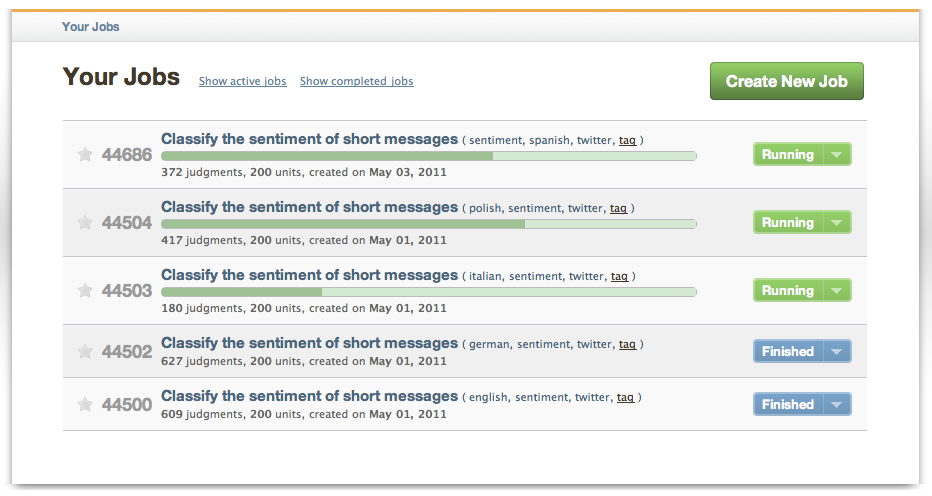
\includegraphics[width=0.8\textwidth]{crowdflower-jobs.png}
    \caption{List of running and finished jobs -- CrowdFlower}
    \label{fig:crowdflower-jobs}
  \end{center}
\end{figure}

In order to generate sample data, a new \verb|Classifier::Crowdflower| class was introduced, which shares the basic infrastructure with the rest of the classifiers, with the exception of the evaluation, which was handled manually. This class outputs several CSV\footnote{Comma-separated values} files, in the format which can then be imported into Crowdflower. Each file contains 200 messages, equally divided between both polarities, for a total of 5 files containing 1,000 tweets selected for manual verification.

CrowdFlower provides an online editor (see Figure \ref{fig:crowdflower-editor}) which allows to create and test tasks before they are distributed to remote workers. Since I was trying to verify two separate assumptions (language and sentiment filter confidence), users were presented with two questions per tweet, along with a note describing the task and clarifying individual questions as necessary:

\begin{quote}
  \textbf{Classify the sentiment of sort messages.} Please read the messages below and, for each of them, confirm which language it is written in and determine whether the attitude of the speaker is positive, negative or neutral.

  \begin{enumerate}
    \item \textbf{Language:} English, Spanish, German, Italian, Polish. \\ \textit{If the message is written in more than one language, please try to determine which is the primary language of the message. E.g. `I love fu{\ss}ball' shall be considered English, even though it contains German words. Similarly `Ich liebe football' would be considered German.}
    \item \textbf{Sentiment:} Neutral, Positive, Negative.
  \end{enumerate}
\end{quote}

\begin{figure}[htb]
  \begin{center}
    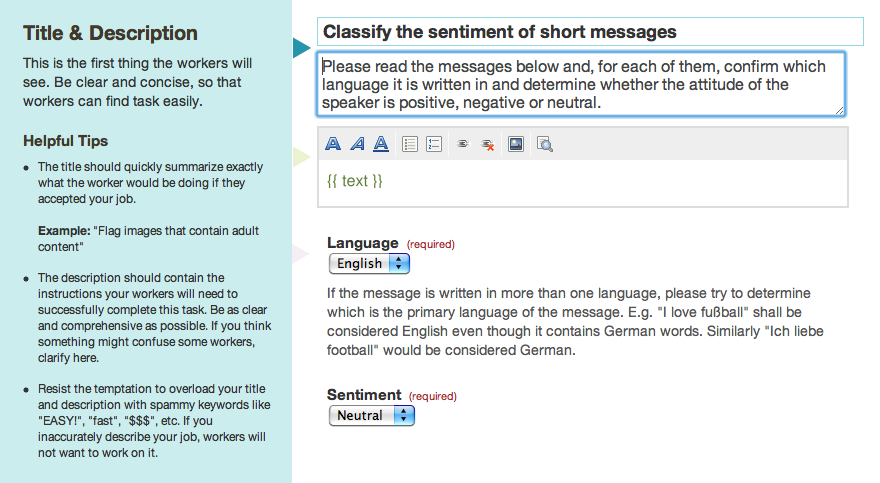
\includegraphics[width=0.8\textwidth]{crowdflower-editor.png}
    \caption{Visual job request editor -- CrowdFlower}
    \label{fig:crowdflower-editor}
  \end{center}
\end{figure}

Certain location requirements (see table below) were also imposed on workers in order to minimise the risk of them not speaking the language in which the message they are evaluating was written. Each job was also tagged with certain keywords (\verb|language|, \verb|sentiment|, \verb|twitter|, \verb|attitude| and \verb|tweet|) which help match workers to tasks they feel comfortable doing.

\begin{center}
  \begin{tabular}{ | l | l | }
    \hline
      {\bf Language} & {\bf Location} \\
    \hline
      English & United Kingdom \\
      Spanish & Spain \\
      German & Germany \\
      Italian & Italy \\
      Polish & Poland \\
    \hline
  \end{tabular}
\end{center}

Ordered jobs are then distributed to workers in selected countries using four different delivery channels (Amazon's Mechanical Turk\footnote{\url{http://www.mturk.com}}, Gambit\footnote{\url{http://www.getgambit.com/}}, Give Work\footnote{\url{http://www.samasource.org/iphone}} and CrowdFlower's internal interface). Each worker is then presented with an interface allowing them to make up to 50 judgements as illustrated in Figure \ref{fig:crowdflower-worker}.

\begin{figure}[htb]
  \begin{center}
    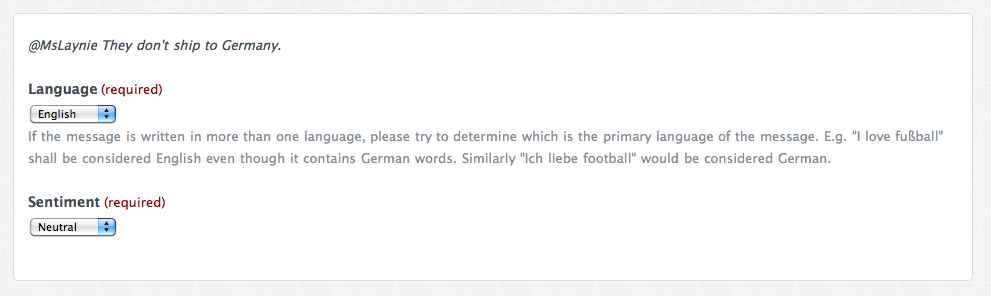
\includegraphics[width=0.8\textwidth]{crowdflower-worker.png}
    \caption{Survey interface for individual workers -- CrowdFlower}
    \label{fig:crowdflower-worker}
  \end{center}
\end{figure}

Workers are remunerated depending on the number of judgements they make for a predefined price per task. Evaluation of our sample of 1,000 units and 3,000 judgements costs under \$60, making CrowdFlower an appealing alternative to carrying out surveys, which would take hours of researchers' time. However, despite CrowdFlower's focus on large-scale data, evaluating a relatively small sample took over two weeks. This level of performance was acceptable in the scope of this project, but might not be for someone trying to replicate the results in a shorter timeframe.

\subsection{Results}

CrowdFlower delivers the results in two different formats--full and aggregated--both in form of a CSV spreadsheet (see Figure \ref{fig:crowdflower-results}). In case of the former, each row represents an individual judgement made by a worker for a given tweet. Since individual tweet will have multiple (at least 3) judgements, I prefer to use the aggregated summary where multiple judgements are collapsed down and a confidence score is given to represent workers' agreement on the sentiment and language of each tweet.

\begin{figure}[htb]
  \begin{center}
    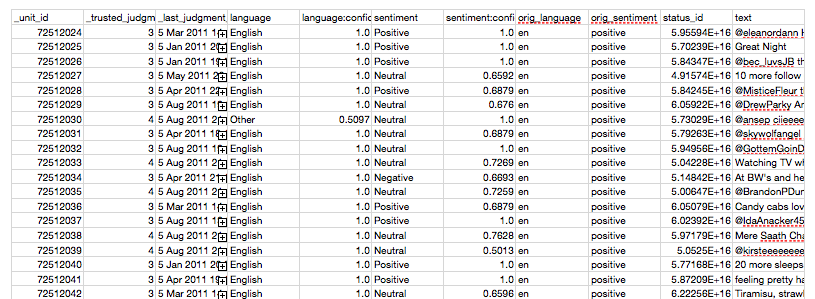
\includegraphics[width=0.8\textwidth]{crowdflower-results.png}
    \caption{Aggregated results for English -- CrowdFlower}
    \label{fig:crowdflower-results}
  \end{center}
\end{figure}

Calculations normally handled by \verb|Classifier::Base| through the \verb|Score| class have been carried out using desktop spreadsheet software, in this case Apple Numbers (part of the iWork\footnote{http://www.apple.com/iwork/} productivity suite), in order to avoid having to import augmented CSV files back into the project.

\section{Summary}

In this chapter I described how the infrastructure for evaluating different classifiers was implemented, how test and training data was collected and how the assumptions about the data set were evaluated. The latter is an extension which had not been part of the original proposal and was completed instead of focusing on implementing a sample application or an API, as suggested in the Overseers' Report. This provided invaluable insight into the quality of data gathered and how it relates to the overall performance of evaluated algorithms.